\pdfoutput=1
\documentclass[11pt,a4paper]{article}

\usepackage[utf8]{inputenc}
\usepackage[a4paper,margin=2.5cm]{geometry}
\usepackage{amsmath,amssymb}
\usepackage{graphicx}
\usepackage{booktabs}
\usepackage{array}
\usepackage{tabularx}
\usepackage{multirow}
\usepackage{microtype}
\usepackage[round,authoryear]{natbib}
\usepackage{xcolor}
\usepackage{tikz}
\usetikzlibrary{positioning,decorations.pathreplacing,calc}
\usepackage[most]{tcolorbox}
\usepackage{caption}
\usepackage{enumitem}
\usepackage{placeins}
\usepackage{eurosym}
\usepackage{url}
\usepackage{xurl}
\usepackage[hidelinks]{hyperref}
\usepackage[nameinlink,capitalise,noabbrev]{cleveref}

\definecolor{cbase}{HTML}{2A78D6}
\definecolor{cacc}{HTML}{EB6834}
\definecolor{chigh}{HTML}{1BAF7A}
\definecolor{ink2}{HTML}{52514E}
\definecolor{rule}{HTML}{D8D7D2}
\definecolor{panel}{HTML}{F4F3EF}
\hypersetup{colorlinks=true,linkcolor=cbase!80!black,citecolor=cbase!80!black,urlcolor=cbase!80!black}

\captionsetup{font=small,labelfont=bf,labelsep=colon,skip=6pt}
\captionsetup[table]{position=top}
\setlist{itemsep=2pt,topsep=4pt}
\renewcommand{\arraystretch}{1.12}
\newcommand{\Cfi}{C_{\mathrm{FI}}}
\newcommand{\CN}{C_{\mathrm{N}}}
\newcommand{\sFI}{s_{\mathrm{FI}}}
\newcommand{\sourcenote}[1]{\par\vspace{3pt}{\footnotesize\color{ink2}#1\par}}

\title{\textbf{Quantum Computing as an Emerging Electricity Load in Finland}\\[4pt]
\large Scenarios to 2050 and Power-System Implications}
\author{Juhani Merilehto\thanks{The analysis and views expressed are solely those of the author and do not represent any employer or affiliated institution.}}
\date{October 2026}

\begin{document}
\maketitle
\vspace{-1.2em}
\begin{center}\small\color{ink2}Copyright \textcopyright{} 2026 Juhani Merilehto. Text, figures, and data are licensed under CC BY 4.0.\end{center}

\begin{abstract}
\noindent Quantum computing may remain a specialised accelerator, or it may become a material category of electricity-intensive infrastructure. This paper extends a scenario framework for Finland from 2035 to 2050. Electricity is accounted for at a full-stack facility boundary (quantum hardware, modality-specific environment, control, directly induced classical co-compute and dedicated infrastructure) rather than per qubit. The capacities themselves are assumed deployment stress scenarios, not estimates derived from quantum workloads. The 2030 and 2035 planning states of the earlier study are retained. After 2035, Nordic capacity grows toward stated targets subject to annual build limits, commissioning lags, retirement and an explicit Finnish connection budget.

In 2050 the Base case remains a specialised load of 40--800~MW (0.2--5.4~TWh/yr). The Accelerated case reaches 0.5--5~GW (2.1--33.9~TWh/yr) and the High case 1.8--8~GW (6.8--54.3~TWh/yr). Fingrid's long-horizon scenarios place Finnish consumption in 2045 at 131--359~TWh; against that range the High central state of 32.3~TWh corresponds to roughly 9--25\% of national demand, and it exceeds the expected electricity use of all data-centre projects holding signed Finnish connection agreements in 2026 combined. At that scale quantum-related demand is no longer a connection-queue question but a matter of system adequacy and the national electricity balance.

Under the assumed targets, timing mainly reshapes intermediate deployment, but a genuine five-year delay lowers the High central 2050 result by about one-sixth. The High central state sits where target, hosting share and connection budget coincide. A present-system-like operating floor would leave 3.5--5.5~GW of the High states in place through scarcity hours. Connected capacity, minimum stable import and physical hosting, not qubit counts, remain the variables to track.
\end{abstract}

\begin{tcolorbox}[enhanced,colback=panel,colframe=panel,arc=2pt,boxrule=0pt,left=8pt,right=8pt,top=6pt,bottom=6pt,
  title={\textbf{Key findings}},coltitle=black,fonttitle=\small,attach title to upper={\par\vspace{2pt}}]
\small
\begin{itemize}[leftmargin=12pt]
  \item \textbf{2035 is a connection question; 2050 can be a system question.} The 2035 envelopes span 5~MW to 2.5~GW. By 2050 the Accelerated and High central states reach 2.1 and 6~GW of Finnish connected capacity, and 12 and 32~TWh per year.
  \item \textbf{Materiality has a threshold.} The Base case stays at or below about 5\% of any published national scenario. The Accelerated upper and High central states reach one-tenth to one-quarter of Fingrid's 2045 range, more than the projected use of all data-centre projects holding signed connection agreements in 2026.
  \item \textbf{The endpoint follows targets, hosting and connection budget, but timing still matters.} With transitions normalised to the 2050 targets, midpoints and lags change only the path. A genuine delay of 5 or 10 years lowers the High central 2050 result by 17\% or 48\%. In four of nine paired states the connection budget is at or below requested hosting.
  \item \textbf{Stickiness is an independent risk axis.} At the High upper capacity, raising the minimum-stable fraction from 25\% to 78\% lifts the operating floor from 1.8 to 5.5~GW at an unchanged 7.0~GW peak.
  \item \textbf{Rebound can be limited by the connection itself.} If half of the withheld energy is recovered, a four-hour curtailment of the High upper span needs roughly 6--11 hours to recover within the headroom above mean or peak operation, and longer if part of that headroom is reserved for redundancy.
\end{itemize}
\end{tcolorbox}

%=====================================================================
\section{Introduction}
%=====================================================================
Quantum computing is increasingly discussed alongside AI and advanced data-centre infrastructure, but its electricity-market implications are structurally different from the more mature data-centre problem. Quantum processors are not another class of server that can be translated into a standard rack density. The grid-facing load is created by a heterogeneous technical stack: the quantum processor itself, refrigeration or vacuum systems, lasers and optics for some modalities, control and readout electronics, classical computing for orchestration and error correction, and conventional facility infrastructure. The composition of that stack can change substantially as the technology scales.

Finland remains a useful case study, and its electricity market is undergoing a demand-led transformation in which data centres are the most visible driver \citep{merilehto2026blog}. The country combines a domestic superconducting-quantum ecosystem, major HPC infrastructure, low-carbon electricity, and a power system facing a very large queue of new electricity-intensive projects. Since the earlier study to 2035 \citep{merilehto2026qc2035}, that queue has grown further. Fingrid now reports nearly 5~GW of data-centre projects with signed connection agreements and more than 145~GW of connection enquiries, about 100~GW of them from data centres \citep{fingrid2026prospects}. If every agreed connection project were realised, Finnish consumption could rise by as much as 40\% from its 2025 level \citep{fingrid2026q3}.

The earlier study concluded that quantum computing is primarily a project-scale connection issue through 2030 and could become material to the national balance only in the upper 2035 states. A 2050 horizon allows that conclusion to be tested properly: whether successful fault-tolerant quantum computing (FTQC) could plausibly be replicated into a large Finnish load, what would have to be true for that to happen, and how large the load would be relative to the national system. The paper therefore retains the four questions of the earlier study and extends them to 2050:
\begin{enumerate}
  \item What consumes electricity in a quantum-computing facility, and how does the load differ across technology modalities?
  \item How does quantum-compute flexibility differ from conventional hyperscale, AI-training and inference loads?
  \item What 2035--2050 electricity-demand envelopes are useful for Finnish grid and market planning, without pretending that qubit roadmaps map directly into MW?
  \item Under what conditions does quantum computing move from a local connection issue to a nationally material electricity-demand category?
\end{enumerate}
The analysis is scenario-based rather than probabilistic. The cases are conditional planning envelopes, not forecasts with assigned probabilities. Public-source information was reviewed through 29 October 2026.

%=====================================================================
\section{Evidence base and horizon selection}
%=====================================================================
\subsection{The observable Finnish and Nordic deployment path}
The most defensible near-term evidence is still physical deployment. VTT operates VTT~Q50, a superconducting system specified at 53 qubits, co-developed with IQM in Espoo and connected to the LUMI supercomputer. VTT and IQM plan a 150-qubit system in 2026 followed by a 300-qubit system at a later stage \citep{vtt2026infra,vtt2025iqm300}. CSC's LUMI-IQ, hosted in Kajaani, is now scheduled for staged delivery: an IQM Halocene~H4 system with 150 physical qubits and initial error correction in 2027, error-correction upgrades in 2028, and a final upgrade to a Halocene~H5 system in 2029. It is described as designed from the start to operate with logical qubits \citep{csc2026lumiiq}. Elsewhere in the Nordics, QuNorth's Magne is planned for early 2027 with roughly 50 logical qubits on more than 1,200 neutral-atom physical qubits \citep{qunorth2026magne}, and Chalmers' WACQT programme targets a 100-qubit superconducting machine by 2030 \citep{chalmers2026}. The common architecture is hybrid: quantum processors act as specialised accelerators inside broader classical-compute workflows.

None of these announcements discloses a grid-MW figure. The best direct anchor remains a measured one: \citet{carrasco2026energy} report a steady-state power of $21.4\pm2.4$~kW for CESGA's deployed 32-qubit QMIO machine, including its dedicated cryogenics, control electronics, classical processing and water-cooling chiller. The measurement is not a whole-building, PUE-adjusted grid meter, and no generic overhead multiplier is applied here.

The paper keeps the strict incremental-attribution rule of the earlier study. Existing HPC or AI capacity is not relabelled as quantum demand merely because a QPU is attached to it. That rule is becoming more important, not less. Quantinuum has announced that its Helios system will be deployed inside an Oracle Cloud Infrastructure AI data centre \citep{quantinuum2026q2}; once QPUs sit inside AI campuses, the site meter and the quantum-attributable increment diverge by construction. As in the earlier study, the 2030 Base envelope (0.5--7~MW) is therefore intentionally dominated by directly induced classical co-compute, dedicated cooling and power infrastructure, redundancy and connection headroom rather than by QPU-system power. Two to three present-system equivalents at 20--50~kW each contribute only about 0.04--0.15~MW.

\subsection{Technology anchors for 2030--2045}
Public roadmaps place the first large fault-tolerant machines at the end of this decade and their successors in the early 2030s. IBM targets Starling in 2029 (200 qubits running $10^8$ gates) and Blue Jay from 2033 (2,000 qubits running $10^9$ gates) \citep{ibm2026roadmap}. Quantinuum reported in August 2026 that Sol remains planned for 2027 and that Apollo, its universal fault-tolerant system, remains on schedule for 2029 \citep{quantinuum2026q2}. PsiQuantum has broken ground on a site in Chicago intended to host a million-qubit-scale fault-tolerant machine, and is building a utility-scale site in Brisbane with ``modular infrastructure similar to a modern data centre'', more than a hundred cryogenic cabinets and a dedicated cryoplant \citep{psiquantum2025chicago,bea2025psiq}. Neither site discloses an electrical capacity.

Resource studies indicate what utility-scale workloads might require. Co-designed chemistry problems are estimated to need roughly 0.75--5.7 million physical qubits and one to nine days of runtime, depending on modality and problem size \citep{gratsea2025codesign}. On the electrical side, \citet{santos2026spin} estimate about 100~kW for a fault-tolerant spin-qubit system of about one million physical qubits, with control demultiplexing reducing energy cost by roughly two orders of magnitude. \citet{mccollum2026futures}, by contrast, estimate the quantum-related portion of superconducting FTQC configurations with about $2\times10^5$ to $2\times10^7$ physical qubits (after doubling for error correction) at roughly 4--27~MW per machine, excluding classical compute, and identify helium-3 and water rather than electricity as the likely bottlenecks to large-scale deployment. These estimates are not comparable to one another or to a site meter, but together they span almost two orders of magnitude per machine: depending on modality and architecture, a commercially useful machine may draw around 100~kW or more than 10~MW.

For the scenario construction, the anchors motivate one assumption. Replicated commercial infrastructure follows first-of-a-kind FTQC by roughly one to two hardware generations. The post-2035 transition midpoints are therefore placed at 2040 (High), 2042 (Accelerated) and 2044 (Base), seven to eleven years after the earliest Blue~Jay-class date. \Cref{sec:robust} shows that moving these midpoints by $\pm3$ years changes the 2040 and 2045 checkpoints but not the 2050 endpoints, because the transition is normalised to the 2050 targets. A genuine delay that shifts the whole transition later is tested separately and does lower the endpoints.

\subsection{Why 2050, and what the horizon can and cannot support}
The earlier study argued that MW estimates beyond 2035 ``would create more apparent precision than information'' \citep{merilehto2026qc2035}. That caution still applies to point estimates. It does not apply to the planning question this paper asks: \emph{if} the 2035 states are reached and replication continues, which constraints determine Finnish load by 2050, and how large can it become before the national system has to plan for it? Answering that question requires three changes to the method rather than a longer extrapolation.

First, post-2035 growth is constructed explicitly: capacity is ordered, commissioned, retired and hosted, and each step has a stated limit. Second, intermediate checkpoints for 2040 and 2045 are reported, because the path matters for connection sequencing even where the endpoint does not. Third, the robustness of the endpoint to every construction parameter is tested (\cref{sec:robust}). The 2050 values in the text are rounded; the supporting data retain full precision only so that the arithmetic can be audited.

\subsection{Finnish power-system scale}\label{sec:scale}
Finnish consumption was about 84.5~TWh in 2025 and grew 5.0\% year-on-year in January--September 2026 \citep{fingrid2026q3}. Fingrid's Q3/2026 outlook places annual consumption at 106--123~TWh in 2030 and 110--162~TWh in 2035, revised upward mainly because of data centres \citep{fingrid2026prospects}. The same outlook gives data-centre consumption of 9--18~TWh in 2030 and 11--35~TWh in 2035. It estimates that the data-centre projects holding connection agreements by mid-August 2026 would consume about 28~TWh if all were built, converting nominal capacity to energy at 65\% average utilisation. Announced Finnish data-centre projects sum to more than 11~GW of nominal capacity at their maximum, of which about 4.5~GW is under construction, nearly three times the capacity of Olkiluoto~3; signed data-centre connection agreements rose from about 3~GW to nearly 5~GW between June and August 2026 alone \citep{merilehto2026blog}. Campuses are built in phases, and nominal capacity does not mean continuous consumption, which is the same distinction between connected capacity, realised peak and annual use that this paper applies to quantum facilities.

No official 2050 projection exists. The longest published Finnish horizon is Fingrid's electricity system vision, whose four scenarios place 2045 consumption at 131~TWh (Local Power), 219~TWh (Windy Seas), 273~TWh (Power to Products) and 359~TWh (Hydrogen from Wind) \citep{fingrid2023vision}. This paper uses that 131--359~TWh range as its long-horizon national scale reference, and the Q3/2026 range for 2035 as a nearer one. Neither is a forecast of the 2050 system; both say whether a quantum-related load is small or large relative to the futures Finnish system planners actually discuss.

For capacity, the reference points are the all-time consumption record of 15,553~MW from January 2026 \citep{fingrid2026q1} and the nearly 5~GW of data-centre capacity under signed agreements. Adequacy is already tight. Fingrid estimates that Finland will need about 1,000~MW of weather-independent production capacity by the turn of the decade \citep{fingrid2026q3}, and that several gigawatts of new dispatchable capacity would be required by 2035 in its High Growth scenario \citep{fingrid2026prospects}.

%=====================================================================
\section{From quantum computer to electrical load}
%=====================================================================
\subsection{A full-stack electricity boundary}
A quantum computer should not be modelled as a QPU alone. Full-system energy studies emphasise that the relevant boundary includes both quantum and classical hardware and that cloud services rarely expose cryogenic and control overheads directly \citep{niu2026full,carrasco2026energy}. For grid analysis, the site meter can be written conceptually as
\begin{equation}\label{eq:meter}
P_{\mathrm{meter}}(t) = P_{\mathrm{QPU}}(t) + P_{\mathrm{env}}(t) + P_{\mathrm{ctrl}}(t) + P_{\mathrm{classical}}(t) + P_{\mathrm{facility}}(t) + P_{\mathrm{other\,campus}}(t),
\end{equation}
where $P_{\mathrm{env}}$ represents modality-specific refrigeration, vacuum, laser or optical infrastructure, $P_{\mathrm{ctrl}}$ represents control and readout, and $P_{\mathrm{classical}}$ includes compilation, orchestration, decoding and other directly coupled compute. The final term captures non-quantum campus loads and is not attributed to quantum computing.

\begin{figure}[t]
\centering
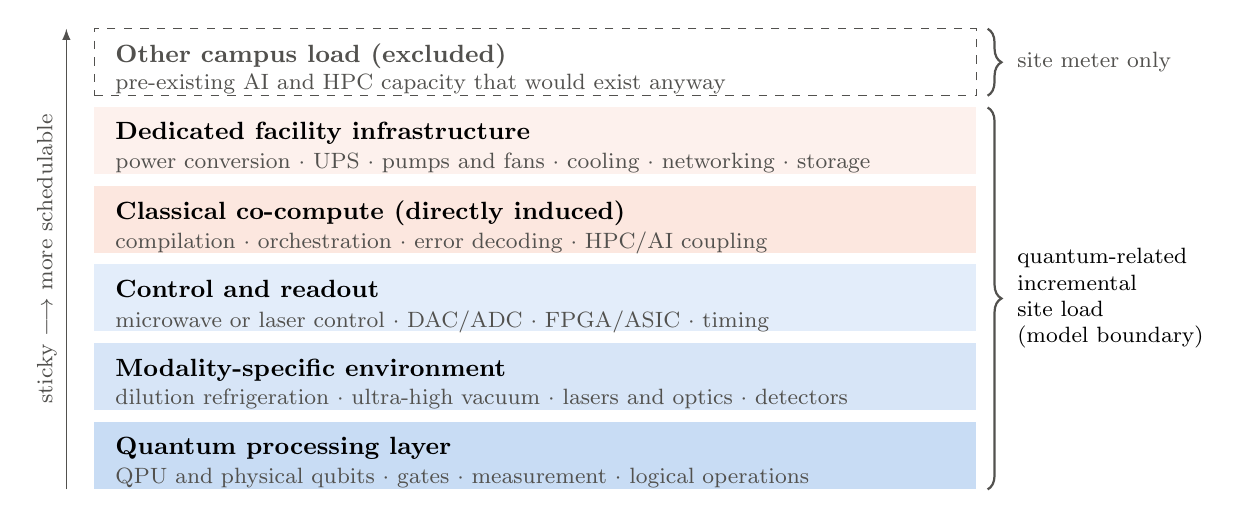
\begin{tikzpicture}[
  layer/.style={draw=none,fill=#1,minimum height=8.5mm,anchor=south west,inner sep=0pt},
  ttl/.style={font=\small\bfseries,anchor=north west,text=black},
  sub/.style={font=\footnotesize,anchor=north west,text=ink2},
  x=1cm,y=1cm]
\def\W{11.2}
\foreach \i/\c/\t/\s in {
  0/cbase!26/Quantum processing layer/QPU and physical qubits $\cdot$ gates $\cdot$ measurement $\cdot$ logical operations,
  1/cbase!19/Modality-specific environment/dilution refrigeration $\cdot$ ultra-high vacuum $\cdot$ lasers and optics $\cdot$ detectors,
  2/cbase!13/Control and readout/{microwave or laser control $\cdot$ DAC/ADC $\cdot$ FPGA/ASIC $\cdot$ timing},
  3/cacc!16/Classical co-compute (directly induced)/{compilation $\cdot$ orchestration $\cdot$ error decoding $\cdot$ HPC/AI coupling},
  4/cacc!9/Dedicated facility infrastructure/power conversion $\cdot$ UPS $\cdot$ pumps and fans $\cdot$ cooling $\cdot$ networking $\cdot$ storage}
{
  \node[layer=\c,minimum width=\W cm] (L\i) at (0,{\i*1.0}) {};
  \node[ttl] at ($(L\i.north west)+(0.15,-0.08)$) {\t};
  \node[sub] at ($(L\i.north west)+(0.15,-0.47)$) {\s};
}
\node[draw=ink2,dashed,fill=white,minimum width=\W cm,minimum height=8.5mm,anchor=south west,inner sep=0pt] (L5) at (0,5.0) {};
\node[ttl,text=ink2] at ($(L5.north west)+(0.15,-0.08)$) {Other campus load (excluded)};
\node[sub] at ($(L5.north west)+(0.15,-0.47)$) {pre-existing AI and HPC capacity that would exist anyway};
\draw[decorate,decoration={brace,amplitude=5pt},thick,ink2] (\W+0.15,4.85) -- (\W+0.15,0.0)
  node[midway,right=7pt,font=\footnotesize,align=left,text=black] {quantum-related\\incremental\\site load\\(model boundary)};
\draw[decorate,decoration={brace,amplitude=5pt},thick,ink2] (\W+0.15,5.85) -- (\W+0.15,5.0)
  node[midway,right=7pt,font=\footnotesize,align=left,text=ink2] {site meter only};
\draw[ink2,-latex] (-0.35,0) -- (-0.35,5.85) node[midway,rotate=90,above,font=\footnotesize,text=ink2] {sticky $\longrightarrow$ more schedulable};
\end{tikzpicture}
\caption{Grid-facing demand anatomy and the modelling boundary. Block heights are conceptual, not component shares. Hardware modality redistributes the lower three layers; at large scale the classical and facility layers can dominate the attributable load. Architecture synthesised from \citet{martin2022energy}, \citet{fellous2023optimizing}, \citet{niu2026full}, \citet{carrasco2026energy} and \citet{ibm2026hardware}.}
\label{fig:anatomy}
\end{figure}

\Cref{fig:anatomy} summarises the boundary. The modelling quantity used throughout is \emph{quantum-related incremental site load}: the electrical capacity that would plausibly not have been built in Finland without the quantum deployment. It includes dedicated support and directly coupled classical compute, but not an entire pre-existing AI/HPC campus merely because a QPU is installed there. The boundary is intentionally narrower than the grid meter and broader than the QPU.

\subsection{Empirical power anchors across modalities}
Present-day measurements and hardware-aware reference architectures prevent a category error between machine power and future site capacity. \Cref{tab:anchors} shows that representative present-day systems are in the order of tens of kilowatts, while the internal source of that demand differs materially by platform. The two projected fault-tolerant estimates differ by about two orders of magnitude per machine, which is itself a measure of how open the large-scale electricity question remains.

\begin{table}[t]
\centering
\caption{Order-of-magnitude electricity anchors for current, near-current and projected fault-tolerant architectures.}
\label{tab:anchors}
\small
\begin{tabularx}{\linewidth}{@{}p{3.6cm}p{2.2cm}X@{}}
\toprule
System / modality & Approx.\ power & Boundary and dominant components \\
\midrule
CESGA QMIO, 32 superconducting qubits & $21.4\pm2.4$~kW & Directly measured deployed-system steady state, including cryogenics, control, classical processing and dedicated chiller; cooling about 76\% of total. Shared building services not identified. \\
Superconducting reference, $\sim$50 qubits & $\sim$20~kW & Hardware-aware reference; cryogenic cooling about 16.1~kW ($\sim$80\%); control/readout roughly 1~kW. \\
Trapped-ion reference, $\sim$10 qubits & $\sim$10~kW & Room-temperature single-gate-zone reference; similar order expected at $\sim$100 qubits; facility HVAC about 78\%. \\
Neutral-atom reference, $\sim$400 qubits & $\sim$22~kW & Qubit-control equipment including laser chillers about 65\%; environment/HVAC most of the remainder. \\
Spin-qubit FTQC estimate, $\sim$$10^6$ physical qubits & $\sim$100~kW & Modelled total including cryostat (5--10~kW input), control instrumentation with 1:500 demultiplexing, and auxiliaries \citep{santos2026spin}. Projected, not measured. \\
Superconducting FTQC configurations, $\sim$$2\times10^5$ to $2\times10^7$ physical qubits & $\sim$4--27~MW per machine & Quantum-related portion only: control, cryogenics including cryoplant, cooling water, plus 20\% for baseload IT and miscellaneous loads; classical compute excluded \citep{mccollum2026futures}. Projected, not measured. \\
\bottomrule
\end{tabularx}
\sourcenote{Source: \citet{carrasco2026energy} for the first four rows; \citet{santos2026spin} and \citet{mccollum2026futures} for the last two. Qubit counts differ by orders of magnitude; the table is not a per-qubit efficiency comparison or a scaling law.}
\end{table}

The modelling implication is explicit. A 100~MW or 1~GW scenario is not a claim that a QPU consumes that much power. Multi-megawatt envelopes require aggregation across systems and, increasingly, quantum-attributable classical co-compute, redundancy, power conversion, cooling and networking. \Cref{sec:intensity} quantifies how far the 2050 envelopes must rely on those surrounding layers.

\subsection{Hardware modality matters}
There is no single quantum electricity architecture. Superconducting systems require dilution refrigeration at millikelvin temperatures and extensive microwave control and readout. Semiconductor spin systems are also generally cryogenic, although higher operating temperatures and on-chip demultiplexing could change refrigeration and control needs materially \citep{santos2026spin}. Trapped-ion and neutral-atom systems shift the burden toward ultra-high vacuum, lasers, optical control and atom or ion handling. Photonic systems depend on sources, detectors, interferometers and control electronics, with cryogenic detection in some architectures; PsiQuantum's planned sites centre on a large cryoplant serving many cabinets \citep{bea2025psiq}. A 2026 cross-platform study concludes that one universal energy model is not appropriate \citep{carrasco2026energy}.

Scaling also changes the internal balance. Superconducting FTQC is expected to need a heterogeneous quantum--classical architecture in which some control electronics migrate toward cryogenic stages \citep{kawabata2026cryo}. The relevant metric is therefore not MW per physical qubit, but electrical input per unit of useful computation delivered by the entire stack.

\subsection{Why current systems look electrically ``always on''}
Total quantum-system power can change little between active computation and idle operation because large support components remain energised; current systems can be left running for months after initialisation \citep{carrasco2026energy}. Deferring a quantum job does not necessarily produce a proportional reduction at the grid meter. Full shutdown is also slow: commercial dilution-refrigerator specifications show empty-system cooldown times from under 12 hours to around a day, and loaded systems depend on added mass and thermalisation \citep{bluefors2026dr,bluefors2026sd}. For present cryogenic architectures, a full thermal cycle should not be treated as sub-hour demand response.

%=====================================================================
\section{Operational flexibility and comparison with data centres}
%=====================================================================
\subsection{Compute flexibility is not electrical flexibility}
Site power can be decomposed into a relatively sticky component and a dispatchable component:
\begin{equation}\label{eq:decomp}
P_{\mathrm{site}}(t) = P_{\mathrm{sticky}}(t) + P_{\mathrm{sched}}(t) + P_{\mathrm{aux}}(t).
\end{equation}
$P_{\mathrm{sticky}}$ includes loads that are costly or slow to shut down, such as refrigeration, vacuum systems, minimum environmental control and essential infrastructure. $P_{\mathrm{sched}}$ represents computational work that can be queued or shifted, and $P_{\mathrm{aux}}$ other variable facility loads. The maximum usable demand response is bounded by the electrically dispatchable portion, not by the share of jobs that are computationally deferrable. Once $P_{\mathrm{sched}}$ has been curtailed, the short-duration operating floor is approximately $P_{\mathrm{sticky}}+P_{\mathrm{aux,min}}$.

Many target applications, such as materials simulation, chemistry, optimisation and hybrid batch workflows, can be scheduled. Yet if the QPU environment and controls remain energised while a job is paused, the immediate MW reduction may be modest. The strongest flexibility is likely to sit in the classical co-compute layer. \Cref{tab:flex} separates computational schedulability from fast electrical response.

\begin{table}[t]
\centering
\caption{Compute and electrical flexibility by load layer (qualitative).}
\label{tab:flex}
\small
\begin{tabularx}{\linewidth}{@{}p{3.3cm}p{2.0cm}p{2.0cm}X@{}}
\toprule
Load / workload layer & Useful work deferrable? & Fast site-MW reduction? & Primary constraint \\
\midrule
Quantum environment base & N/A & Low & Thermal or vacuum recovery; essential support remains energised. \\
QPU job execution & High & Low--medium & Useful work can pause while idle system power stays high. \\
QPU classical co-compute & High & High & Scheduler, job state and workload migration. \\
AI training workload & Medium--high & Medium--high & Training progress, orchestration, service levels. \\
Latency-critical inference & Low--medium & Medium & Service latency, availability, capacity. \\
\bottomrule
\end{tabularx}
\sourcenote{Synthesis of current quantum-system architecture and data-centre flexibility literature \citep{carrasco2026energy,williams2026flex,majumder2026ramps}.}
\end{table}

\subsection{Comparison with AI training and hyperscale inference}
Quantum facilities should not be assumed to be either more or less flexible than hyperscale data centres; the correct comparison is workload-specific. Recent experiments demonstrate rapid load reduction and sustained curtailment in GPU clusters through workload orchestration \citep{williams2026flex}, while AI data centres can also produce rapid power ramps as workloads change \citep{majumder2026ramps}. A quantum/HPC campus can combine a technically sticky environmental base, highly schedulable quantum jobs and a potentially large classical layer that behaves more like conventional HPC or AI. At the grid interface, large facilities converge on the same engineering questions as other data centres: maximum import, ramp rate, fault ride-through, power quality, redundancy, commissioning profile, backup supply and contractual curtailment. For market simulation, a future facility is better represented by operating states (minimum stable infrastructure, normal compute, high compute, curtailed compute and recovery) than by a synthetic 24-hour load curve.

%=====================================================================
\section{Scenario methodology}\label{sec:method}
%=====================================================================
\subsection{Retained 2035 states and cluster equivalents}
The 2030 and 2035 states of the earlier study are retained unchanged as dated planning assumptions and are read directly from its published parameter file \citep{merilehto2026qc2035}. The 2030 states remain a near-term checkpoint rather than a second scenario set. Nordic quantum-attributable connected capacity $\CN$ is a planning construction, not a sum of named projects. It is interpreted through stylised cluster equivalents, each denoting the incremental connection capacity of a quantum/HPC deployment including its induced classical and facility layers. In 2035 the Base case corresponds to 4--9 facilities at 5--20~MW, the Accelerated case to 6--16 clusters at 75--125~MW, and the High case to 10--20 clusters at 150--300~MW. The 2050 Nordic targets correspond, for example, to eight 100~MW Base equivalents, twenty-four 250~MW Accelerated equivalents or about thirty-eight 400~MW High equivalents. These counts make the envelopes interpretable; they are not identified investments.

\begin{table}[t]
\centering
\caption{Scenario construction: retained 2035 states and 2050 settings (low / central / high paired states).}
\label{tab:construction}
\small\setlength{\tabcolsep}{4pt}
\begin{tabular}{@{}lccc@{}}
\toprule
 & Base & Accelerated & High \\
\midrule
\multicolumn{4}{@{}l}{\emph{Retained 2035 states}} \\
Nordic connected capacity (MW) & 20 / 80 / 180 & 450 / 1,100 / 2,000 & 1,500 / 3,000 / 6,000 \\
Finland hosting share & 25 / 32 / 40\% & 30 / 36 / 40\% & 40 / 40 / 42\% \\
Finland connected capacity (MW) & 5 / 25.6 / 72 & 135 / 396 / 800 & 600 / 1,200 / 2,520 \\
\midrule
\multicolumn{4}{@{}l}{\emph{2050 construction settings}} \\
Nordic target (MW) & 200 / 800 / 2,000 & 2,000 / 6,000 / 12,000 & 6,000 / 15,000 / 30,000 \\
Nordic build limit (MW/yr) & 30 / 120 / 300 & 250 / 750 / 1,500 & 800 / 2,000 / 4,000 \\
Requested Finland share & 20 / 30 / 40\% & 25 / 35 / 45\% & 30 / 40 / 50\% \\
Finnish connection budget (MW) & 150 / 400 / 800 & 1,000 / 2,500 / 5,000 & 3,000 / 6,000 / 8,000 \\
Transition midpoint & 2044 & 2042 & 2040 \\
\bottomrule
\end{tabular}
\sourcenote{All states: commissioning lag 4 / 3 / 2 years, retirement 5 / 4 / 3\% per year, logistic transition scale 4 years. Budgets are scenario constraints on Finnish connection and investment capacity, not official grid limits.}
\end{table}

\subsection{Scenario variables}
The framework separates five quantities that should not be conflated:
\begin{enumerate}
  \item \textbf{Nordic quantum-related connected capacity}, $\CN$: grid-import capacity attributable to physically hosted quantum/HPC deployment across the Nordic region.
  \item \textbf{Finland hosting share}, $\sFI$: Finnish use of cloud quantum services creates Finnish electricity demand only when the physical systems and their incremental support are hosted in Finland.
  \item \textbf{Peak-to-connected ratio}, $r$: realised coincident peak import relative to connection capacity, reflecting engineering headroom, phased commissioning and redundancy.
  \item \textbf{Operating load factor}, $\ell$: annual mean demand divided by realised peak.
  \item \textbf{Minimum-stable fraction}, $m$: the share of realised peak that remains after dispatchable computation is curtailed without a full thermal, vacuum or facility shutdown.
\end{enumerate}
Finnish connected capacity, realised peak, minimum stable import and annual energy follow as
\begin{align}
\Cfi &= \min\{\sFI\,\CN,\; B_{\mathrm{FI}}\}, \label{eq:cfi}\\
P_{\mathrm{peak}} &= \Cfi\, r, \qquad P_{\mathrm{min}} = \Cfi\, r\, m, \label{eq:peak}\\
E_{\mathrm{FI}} &= \Cfi\, r\, \ell \times 8760 / 10^{6}\ \ \text{TWh/yr}, \label{eq:energy}
\end{align}
where $B_{\mathrm{FI}}$ is the Finnish connection budget. Up to 2035 the budget is slack and \cref{eq:cfi} reduces to the earlier study's $\Cfi=\sFI\CN$. A necessary consistency condition is $0\le m\le \ell\le 1$ with $0\le r,\sFI\le1$; the script enforces it before writing any result. The 2035 values of $r$, $\ell$ and $m$ (\cref{tab:params}) are retained into 2050 in the main states, and \cref{sec:robust} tests alternatives. The annual-energy convention assumes that curtailment is infrequent; repeated activation would reduce realised TWh.

The low, central and high columns are paired scenario states, not independent confidence intervals. Capacity, $r$ and $\ell$ rise together within a case while $m$ generally falls, reflecting the assumption that larger commercial facilities have larger schedulable classical layers. That co-variation is contestable and is therefore broken deliberately in \cref{sec:sticky}. The $r\ell$ products in the central states (0.62--0.67) are close to the 65\% average utilisation Fingrid applies to nominal data-centre capacity \citep{fingrid2026prospects}, which provides an external plausibility check on the energy conversion.

\subsection{Capacity construction after 2035}
After 2035 the desired Nordic capacity $D_t$ moves from its 2035 value toward the 2050 target along a normalised logistic transition
\begin{equation}\label{eq:desired}
D_t = \CN^{2035} + \bigl(T_{2050}-\CN^{2035}\bigr)\, \frac{\sigma(t)-\sigma(2035)}{\sigma(2050)-\sigma(2035)},\qquad \sigma(t)=\Bigl[1+e^{-(t-t_{\mathrm{mid}})/w}\Bigr]^{-1},
\end{equation}
with midpoint $t_{\mathrm{mid}}$ and scale $w=4$ years. Commissioned capacity evolves as
\begin{equation}\label{eq:stock}
C_{\mathrm{N},t} = (1-\delta)\,C_{\mathrm{N},t-1} + A_t ,
\end{equation}
where $\delta$ is the retirement fraction and $A_t$ the capacity arriving in year $t$ from orders placed $L$ years earlier. Each order fills the gap between the desired capacity at its delivery date and the projected surviving stock plus the pipeline already in flight, capped by the annual build limit. Orders placed before 2035 for delivery in 2036--2035$+L$ are included, so that a pathway growing into 2035 does not stall artificially while the first post-2035 orders are under construction. Without that pipeline, all central paths would decline in 2036--2037 (High central from 1,200 to 1,106~MW) before recovering; the 2050 endpoints are identical either way. Because \cref{eq:desired} is normalised to reach the target in 2050, shifting $t_{\mathrm{mid}}$ reshapes the path without moving the endpoint. A separate delay test therefore shifts the entire post-2035 transition, including the hosting and budget trajectories, $\Delta$ years later without renormalising it, and orders are placed against the delayed path. Orders already in flight in 2035 were placed against the undelayed path and are still delivered.

The requested Finnish share and the connection budget move from their 2035 values to their 2050 settings along the same transition. When the budget binds, the effective hosting share falls below the requested share, and the two are reported separately.

The resulting capacity envelopes are assumed deployment stress scenarios. They are not derived from quantum workloads or component-level electricity requirements, and the size of the classical co-compute layer that the large states imply is an unvalidated assumption (\cref{sec:intensity}). Connected capacity also includes connection headroom: electricity-consuming equipment corresponds at most to the realised peak $\Cfi r$, while $\Cfi(1-r)$ is reserved capacity rather than load.

\subsection{Scenario definitions}
\textbf{Base -- hybrid integration.} Quantum computing remains primarily a specialised accelerator integrated with public research, HPC and selected industrial compute. Replication continues slowly; large standalone FTQC campuses remain limited.

\textbf{Accelerated -- commercial scaling.} Practical advantage emerges for a broad enough set of workloads to support repeated commercial Nordic clusters. Classical co-compute, control, redundancy and integration become a material share of the footprint, and Finland captures a meaningful share because of its ecosystem and power/HPC advantages.

\textbf{High -- FTQC scale-up and Finnish concentration.} A deliberately demanding boundary scenario: fault-tolerant architectures work at commercially useful scale, manufacturing supports replication, applications justify dedicated capacity, and Finland captures a large share of Nordic hosting. It is not a central forecast. Its upper Nordic target of 30~GW is a boundary stress that \cref{sec:intensity} shows to be extreme.

A \textbf{no-commercial-scale} outcome also remains admissible: useful research and integration continue without the modelled commercial expansion. \Cref{sec:robust} reports a stalled-construction variant as a lower reference.

%=====================================================================
\section{Scenario results}
%=====================================================================
\subsection{Connected capacity: from connection issue to system category}
\Cref{fig:paths} shows the Finnish connected-capacity paths and \cref{fig:envelopes} places the 2035 and 2050 envelopes against three Finnish scale markers. The first marker is the 30~MW threshold above which the KJV2026 draft sets significant system technical requirements for demand facilities. The consultation closed on 21 August 2026 and confirmation is targeted for March 2027, while Fingrid's separate technical requirements for large demand facilities have applied to transmission-connected demand since June 2026 \citep{fingrid2026kjv,fingrid2026large}. The second is the 250~MW conditional connection-agreement model \citep{fingrid2025conditional}. The third is the nearly 5~GW of data-centre capacity under signed agreements \citep{fingrid2026prospects}.

\begin{figure}[t]
\centering
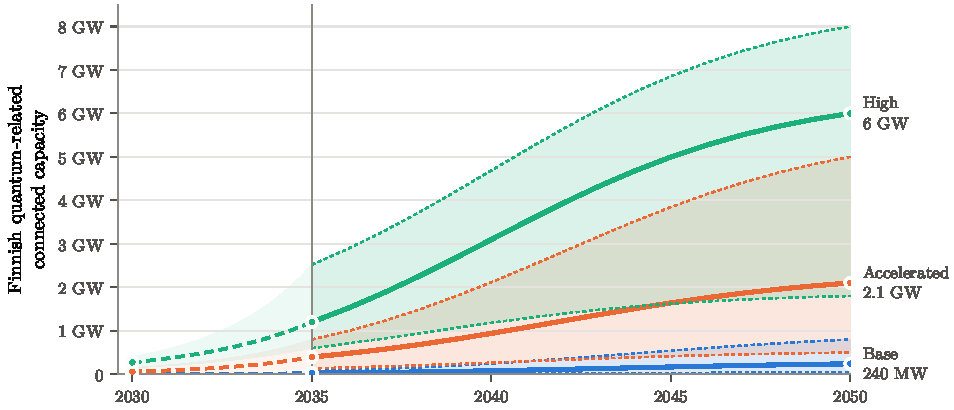
\includegraphics[width=\linewidth]{figures/fig1_paths.pdf}
\caption{Finnish quantum-related connected capacity, 2030--2050, linear scale. Points mark the central 2030 checkpoint and the retained 2035 states; dashed segments connect them illustratively. From 2035, shaded bands span the paired low and high states and solid lines are central states, constructed under the settings of \cref{tab:construction}. Values too small to read at this scale, including all 2030 states and the Base case, are given in \cref{tab:checkpoints}. All paths are planning paths, not annual forecasts.}
\label{fig:paths}
\end{figure}

\begin{figure}[t]
\centering
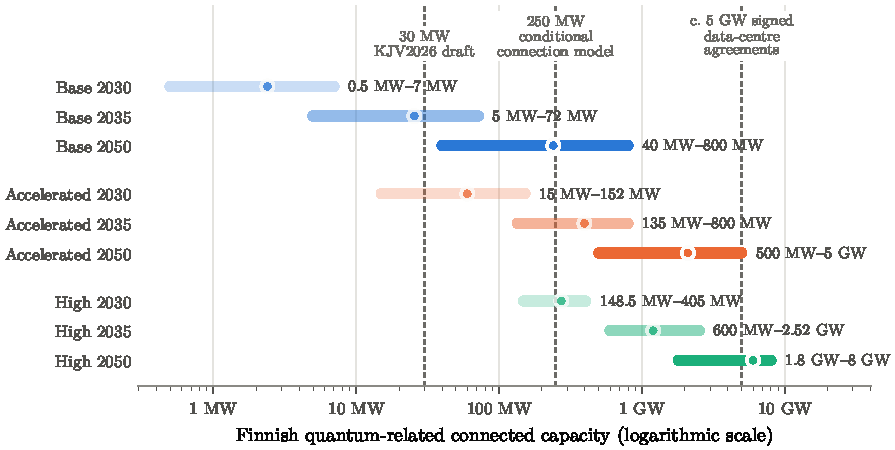
\includegraphics[width=\linewidth]{figures/fig3_envelopes.pdf}
\caption{2030, 2035 and 2050 connected-capacity envelopes against Finnish scale markers. Bars span low to high paired states; points are central states. Markers: KJV2026 draft threshold \citep{fingrid2026kjv}, conditional connection model \citep{fingrid2025conditional}, signed data-centre agreements \citep{fingrid2026prospects}.}
\label{fig:envelopes}
\end{figure}

At the 2030 checkpoint the Base case spans only 0.5--7~MW, the Accelerated case 15--152~MW and the High case 149--405~MW; even the High upper state is about 8\% of today's signed data-centre capacity. By 2035 the Base case remains a specialised-compute issue at 5--72~MW, the Accelerated case is comparable to a major industrial programme at 135--800~MW, and the High case reaches 600--2,520~MW. By 2050 the scale shifts by roughly an order of magnitude. The Base upper state reaches 800~MW, already beyond the conditional-connection threshold. The Accelerated central state reaches 2.1~GW and its upper state 5~GW, equal to today's entire signed data-centre portfolio. The High central state reaches 6~GW. \Cref{tab:checkpoints} reports the 2040 and 2045 checkpoints. In the High central path, more than half of the 2050 capacity is in place by 2040 (3.1~GW) and over 80\% by 2045 (5.0~GW), which is the period in which connection sequencing and reinforcement would have to be decided.

\begin{table}[t]
\centering
\caption{Finnish connected capacity at the checkpoints (MW, low / central / high).}
\label{tab:checkpoints}
\small\setlength{\tabcolsep}{4pt}
\resizebox{\linewidth}{!}{%
\begin{tabular}{@{}lccccc@{}}
\toprule
Case & 2030 & 2035 & 2040 & 2045 & 2050 \\
\midrule
Base & 0.5 / 2.4 / 7 & 5 / 26 / 72 & 15 / 80 / 247 & 30 / 167 / 543 & 40 / 240 / 800 \\
Accelerated & 15 / 60 / 152 & 135 / 396 / 800 & 266 / 940 / 2,115 & 415 / 1,641 / 3,844 & 500 / 2,100 / 5,000 \\
High & 149 / 273 / 405 & 600 / 1,200 / 2,520 & 1,182 / 3,098 / 4,686 & 1,623 / 4,995 / 6,853 & 1,800 / 6,000 / 8,000 \\
\bottomrule
\end{tabular}}
\sourcenote{2030 and 2035: retained states of \citet{merilehto2026qc2035}. 2040 and 2045 values depend on the transition midpoints; see \cref{tab:timing} for $\pm3$-year variants.}
\end{table}

\subsection{Peak import, minimum stable load and annual energy}
\Cref{tab:results} carries connected capacity through to the grid-facing quantities. Realised peak is the quantity to compare with system demand; minimum stable import is the first-order indicator of what remains exposed to scarcity hours after schedulable compute is curtailed; annual energy is relevant for the national balance but substitutes for neither power metric.

\begin{table}[t]
\centering
\caption{Finland scenario results for 2030 and 2035 (retained) and 2050 (low / central / high).}
\label{tab:results}
\small\setlength{\tabcolsep}{3.5pt}
\resizebox{\linewidth}{!}{%
\begin{tabular}{@{}llcccc@{}}
\toprule
Case & Year & Connected (MW) & Realised peak (MW) & Min.\ stable (MW) & Annual (TWh) \\
\midrule
\multirow{3}{*}{Base} & 2030 & 0.5 / 2.4 / 7.0 & 0.33 / 1.8 / 5.95 & 0.26 / 1.37 / 4.28 & 0.002 / 0.014 / 0.046 \\
 & 2035 & 5.0 / 25.6 / 72 & 3.5 / 20.5 / 63.4 & 2.6 / 13.3 / 34.8 & 0.025 / 0.151 / 0.488 \\
 & 2050 & 40 / 240 / 800 & 28 / 192 / 704 & 21 / 125 / 387 & 0.20 / 1.41 / 5.43 \\
\midrule
\multirow{3}{*}{Accelerated} & 2030 & 15 / 60 / 152 & 9.0 / 43 / 125 & 5.9 / 24 / 56 & 0.057 / 0.30 / 0.92 \\
 & 2035 & 135 / 396 / 800 & 88 / 309 / 704 & 48 / 139 / 246 & 0.57 / 2.22 / 5.43 \\
 & 2050 & 500 / 2,100 / 5,000 & 325 / 1,638 / 4,400 & 179 / 737 / 1,540 & 2.11 / 11.8 / 33.9 \\
\midrule
\multirow{3}{*}{High} & 2030 & 149 / 273 / 405 & 82 / 186 / 324 & 45 / 84 / 113 & 0.50 / 1.24 / 2.33 \\
 & 2035 & 600 / 1,200 / 2,520 & 360 / 900 / 2,218 & 162 / 315 / 554 & 2.27 / 6.46 / 17.1 \\
 & 2050 & 1,800 / 6,000 / 8,000 & 1,080 / 4,500 / 7,040 & 486 / 1,575 / 1,760 & 6.81 / 32.3 / 54.3 \\
\bottomrule
\end{tabular}}
\sourcenote{Equations \eqref{eq:cfi}--\eqref{eq:energy} with the operating parameters of \cref{tab:params}. The connection budget binds in the Accelerated and High upper states (effective Finnish shares 41.7\% and 26.7\% against 45\% and 50\% requested) and coincides exactly with requested hosting in the Base upper and High central states.}
\end{table}

\subsection{When does quantum computing become nationally material?}\label{sec:materiality}
This is the question the 2050 horizon is meant to answer. \Cref{fig:materiality} and \cref{tab:materiality} compare the 2050 results with the national and data-centre scale references of \cref{sec:scale}.

\begin{figure}[t]
\centering
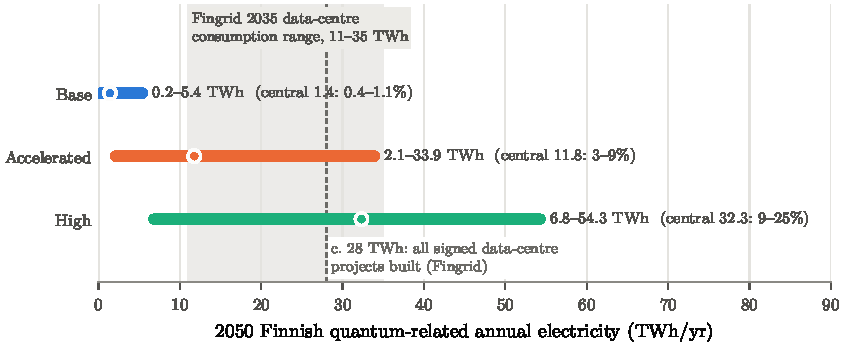
\includegraphics[width=\linewidth]{figures/fig4_materiality.pdf}
\caption{2050 Finnish quantum-related annual electricity against data-centre references. Bars span low to high paired states; points are central states. Percentages express the central state as a share of Fingrid's 2045 scenario range, 131--359~TWh \citep{fingrid2023vision}. The shaded band is Fingrid's 2035 data-centre consumption range and the dashed line the consumption of all data-centre projects with signed agreements if built \citep{fingrid2026prospects}.}
\label{fig:materiality}
\end{figure}

\begin{table}[t]
\centering
\caption{Materiality of 2050 states against present and long-horizon Finnish scale references.}
\label{tab:materiality}
\small\setlength{\tabcolsep}{3.5pt}
\resizebox{\linewidth}{!}{%
\begin{tabular}{@{}lccccc@{}}
\toprule
State & TWh/yr & \% of 2045 range & \% of 2035 range & Peak / 2026 record & $\times$ signed DC energy \\
 & & (131--359~TWh) & (110--162~TWh) & (15,553~MW) & (28~TWh) \\
\midrule
Base central & 1.4 & 0.4--1.1 & 0.9--1.3 & 1.2\% & 0.05 \\
Base upper & 5.4 & 1.5--4.1 & 3.4--4.9 & 4.5\% & 0.19 \\
Accelerated central & 11.8 & 3.3--9.0 & 7.3--10.7 & 10.5\% & 0.42 \\
Accelerated upper & 33.9 & 9.4--25.9 & 21--31 & 28.3\% & 1.21 \\
High central & 32.3 & 9.0--24.7 & 20--29 & 28.9\% & 1.15 \\
High upper & 54.3 & 15.1--41.4 & 34--49 & 45.3\% & 1.94 \\
\bottomrule
\end{tabular}}
\sourcenote{Denominators: \citet{fingrid2023vision} (2045 scenarios), \citet{fingrid2026prospects} (2035 range, data-centre pipeline), \citet{fingrid2026q1} (record). All are present-day or scenario scale anchors, not forecasts of the 2050 system; the 2035 column is shown only as a nearer reference.}
\end{table}

Three thresholds emerge. The Base case stays at or below about 5\% of any published national scenario even in its upper state. It remains a connection and siting issue, larger than in 2035 but not a system category. The Accelerated central state, at about 12~TWh, is comparable to Fingrid's entire 2035 low-end data-centre consumption: material to regional grid planning and visible in the national balance, but within the range that the larger Fingrid scenarios already absorb. The Accelerated upper and High central states, at 32--34~TWh, exceed the expected consumption of all projects holding signed data-centre connection agreements in 2026 (about 28~TWh; Fingrid separately reports about 100~GW of data-centre connection enquiries) and correspond to one-tenth to one-quarter of 2045 national demand, depending on which national future materialises. At that point quantum-related load is not a sensitivity on top of the electrification scenarios; it is one of them. The High upper state, at 54~TWh, would be comparable to the entire 52~TWh spread between Fingrid's Moderate and High Growth outlooks for 2035.

Two qualifications matter. First, materiality depends on which national future occurs: the same 32~TWh is a quarter of a Local Power system and under a tenth of a Hydrogen from Wind system. Second, peak matters more than energy for adequacy. The High central realised peak of 4.5~GW is 29\% of the January 2026 consumption record, in a system that already needs about 1,000~MW of additional weather-independent capacity by the turn of the decade \citep{fingrid2026q3}.

\subsection{Top-down and intensity checks}\label{sec:intensity}
Two checks test whether the envelopes are internally plausible. The first is top-down. The Nordic targets imply Nordic quantum-related electricity of 4.7~TWh (Base central), 33.6~TWh (Accelerated central), 80.8~TWh (High central) and 203.5~TWh (High upper) per year at the corresponding $r$ and $\ell$. For scale, the High central Nordic volume roughly equals Finland's entire 2025 consumption and would be about 7\% of the IEA's 2035 global data-centre benchmark of about 1,200~TWh \citep{iea2025energyai}; global data-centre use was 485~TWh in 2025 and is projected at 950~TWh in 2030 \citep{iea2026keyquestions}. The High upper Nordic volume would be 2.4 times Finland's 2025 consumption and about 17\% of that global benchmark. The earlier study described a 6~GW Nordic state as ``intentionally extreme'' at 3--4\% of the global benchmark; the 30~GW upper target is five times that. It is retained as a boundary stress because the Finnish connection budget, not Nordic demand, sets the High upper Finnish result. It should not be read as a plausible Nordic market size.

The second check concerns intensity, and it shows how far the large states rest on assumptions this paper does not validate. At present-system scale, the High central 6~GW would correspond to some 300,000 systems of about 20~kW. At the fault-tolerant spin-qubit estimate of about 100~kW per million physical qubits \citep{santos2026spin}, it would correspond to roughly $6\times10^{10}$ physical qubits, far beyond any roadmap; in such an architecture almost all of the load would have to be classical co-compute and facility infrastructure. Under the superconducting FTQC configurations of \citet{mccollum2026futures}, by contrast, the quantum-related portion alone is roughly 4--27~MW per machine, or 8--54~MW for a facility with the study's two-machine redundancy. On that basis 6~GW would correspond to about 110--750 such facilities (220--1,500 machines) before any classical compute, and a single 400~MW High cluster equivalent to about 7--50 facilities. That study also estimates that a global helium-3 supply of several tens of thousands of litres per year would allow only around 5--20 fault-tolerant machines to be built per year worldwide, which would constrain a superconducting High pathway well before electricity does.

The multi-gigawatt states are therefore architecture-conditional stress scenarios. They require either very large replication of power-intensive quantum hardware, with its physical-resource constraints resolved, or a quantum-induced classical layer whose size remains unspecified. This paper does not provide a component-level breakdown for a large cluster: the classical-compute share implied by the High states is an assumption, and classical co-compute intensity remains the most important engineering unknown for the High case.

\subsection{Minimum stable demand is an independent risk axis}\label{sec:sticky}
The paired states associate commercial scale with a larger schedulable layer, so the High states are not adequacy-worst cases by construction. \Cref{fig:flex} breaks that pairing. Holding capacity, $r$ and $\ell$ fixed, the minimum-stable fraction is raised to 78\%, calibrated to the high-sticky end of present-system evidence rather than inferred from any single component share.

\begin{figure}[t]
\centering
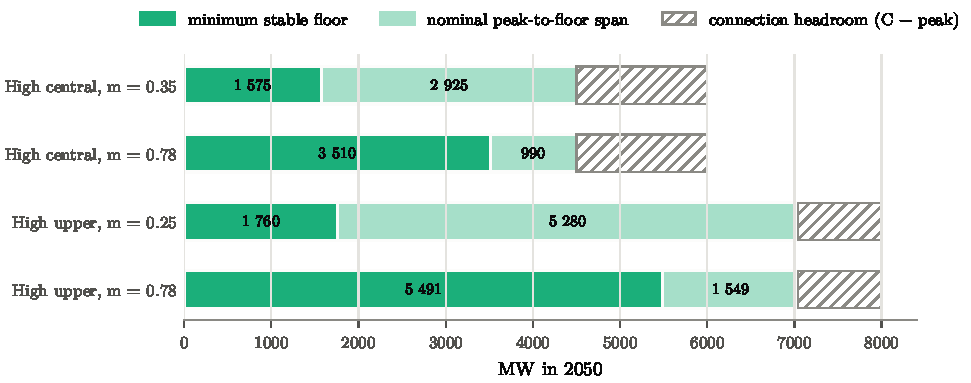
\includegraphics[width=\linewidth]{figures/fig5_flexibility.pdf}
\caption{2050 High central and upper states with paired and sticky minimum-stable fractions. Each bar ends at connected capacity; the hatched segment is connection headroom above realised peak. Annual energy is unchanged across each pair because the normal-use convention is held fixed.}
\label{fig:flex}
\end{figure}

In the High central state the floor rises from 1,575 to 3,510~MW and the nominal peak-to-floor span shrinks from 2,925 to 990~MW. In the upper state the floor rises from 1,760 to 5,491~MW at the same 7,040~MW peak, and the span shrinks from 5,280 to 1,549~MW. Large capacity and low flexibility must therefore be assessed separately unless a project can demonstrate a guaranteed curtailment envelope. The intensity check above points in both directions: a classical-dominated campus may be more flexible than today's systems, but only if its classical layer is designed and contracted for curtailment.

\subsection{Robustness of the 2050 results}\label{sec:robust}
\Cref{fig:tornado} varies each construction and operating parameter one at a time around the High central state. Three results stand out.

\begin{figure}[t]
\centering
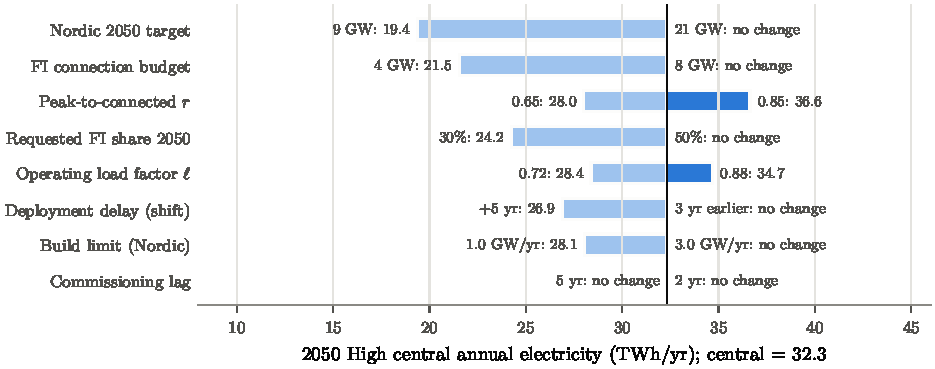
\includegraphics[width=\linewidth]{figures/fig6_tornado.pdf}
\caption{One-way sensitivity of 2050 High central annual electricity. Light bars: low setting; dark bars: high setting. ``No change'' indicates a constraint that does not bind in that direction.}
\label{fig:tornado}
\end{figure}

\emph{First, timing matters, but less than a renormalised test suggests.} Moving the transition midpoint by $\pm3$ years or changing the commissioning lag leaves the 2050 result unchanged. That result is partly built into the construction: the desired path is normalised to reach its target in 2050, and orders anticipate it. Midpoint shifts therefore change the checkpoints instead (High central in 2045: 4.5--5.3~GW, 24--29~TWh; in 2040: 2.5--3.7~GW; \cref{tab:timing}). A genuine delay, which shifts the whole transition later without renormalising it, does move the endpoint (\cref{tab:delay}). Delays of 3, 5 and 10 years lower High central 2050 capacity to 5.5, 5.0 and 3.1~GW (29.7, 26.9 and 16.7~TWh), which reproduces the undelayed 2047, 2045 and 2040 states. The defensible statement is conditional: under the assumed targets, anticipatory ordering and tested build limits, the 2050 level is set by target, hosting and budget, and a delayed commercial breakthrough lowers it by about 8--48\% for delays of 3--10 years.

\emph{Second, the High central state sits on a knife-edge.} Its requested hosting (40\% of 15~GW) equals its 6~GW connection budget exactly, so every upward perturbation of target, share or budget is absorbed by another constraint, while every downward perturbation passes through: a 9~GW Nordic target gives 19.4~TWh, a 30\% share 24.2~TWh, and a 4~GW budget 21.5~TWh. The paired central state is therefore an upper-leaning point within its own construction. Only the operating parameters move it upward: $r=0.85$ gives 36.6~TWh and $\ell=0.88$ gives 34.7~TWh. A slower build limit of 1~GW/yr would leave the target unreached and give 28.1~TWh.

\emph{Third, retained operating parameters are not a hidden optimism.} \Cref{tab:drift} shows that dense utilisation ($r=\ell=0.88$) raises the High central result to 40.7~TWh, while more connection headroom ($r=0.65$) lowers it to 28.0~TWh. Changing $m$ moves the floor between 1.1 and 3.4~GW without changing energy.

Two further variants bound the lower side (\cref{tab:stalled}). If construction stops in 2035 but orders already in flight are delivered, Finnish connected capacity in 2050 is 31~MW (Base), 409~MW (Accelerated) and 1,384~MW (High), or 0.18, 2.3 and 7.5~TWh. If the pipeline is cancelled as well, capacity simply retires to 13, 209 and 651~MW (0.08, 1.2 and 3.5~TWh). A research-only future need not pass through the commercial 2035 states at all, so these are not lower bounds; they show that the commercial cases describe continued investment, not technological momentum.

\subsection{What makes the High case non-linear}
The High case does not assume that every system draws power in proportion to today's hardware. Its non-linearity comes from deployment count and commercial scale, not from deteriorating electricity per useful operation; better error correction, control integration and cryogenic efficiency could reduce it \citep{fellous2023optimizing,carrasco2026energy,santos2026spin}. A high electricity case therefore requires the volume of useful quantum services and installed systems to grow faster than efficiency improves. Four conditions must align: fault-tolerant architectures must work at commercially useful scale; manufacturing and control infrastructure must support replication; applications must justify dedicated capacity against a classical counterfactual; and Finland must capture a large share of Nordic physical hosting within a connection budget that the grid can deliver. Failure of any one leaves global quantum capability high while Finnish electricity demand remains low.

%=====================================================================
\section{Grid and electricity-market implications}
%=====================================================================
\subsection{Grid connection and local reinforcement}
Through 2030 the observable hybrid path remains well below the 30~MW KJV2026 threshold, and only fast commercial and FTQC pathways reach large-demand territory. From the late 2030s, the High central path adds close to 400~MW of Finnish connected capacity per year and the Accelerated central path 100--200~MW (\cref{tab:checkpoints}). If several quantum/HPC clusters concentrate in the same region, aggregate demand can influence reinforcement sequencing in the same way as today's data-centre clusters. A site with excellent cooling, fibre and renewable procurement can still be unattractive if deliverable firm power requires years of network expansion.

Fingrid's current pipeline shows why requested capacity is not a forecast. More than 145~GW of enquiries is roughly nine times the national peak record \citep{fingrid2026prospects}, and the Ministry of Economic Affairs and Employment has published a draft proposal for a priority procedure for grid connections because capacity is insufficient to meet all demand \citep{fingrid2026q3}. Quantum projects should be assessed on the same maturity criteria as other large loads: permitting, land, financing, equipment procurement, credible commissioning and demonstrable use of reserved capacity. Strategic-technology status is not evidence that hundreds of megawatts should be reserved.

\subsection{Scarcity-hour price effects}
Annual TWh is an incomplete predictor of price impact. A large sticky minimum import raises residual demand in every hour, including cold and calm periods, nuclear outages and transmission-constrained situations. In the paired central states, the High case retains about 84~MW after schedulable compute is curtailed in 2030, about 315~MW in 2035 and about 1.6~GW in 2050; in the sticky variant, 3.5~GW. In the Base case the national price effect remains small relative to uncertainty in data centres, electric heating, hydrogen and industrial electrification, even in 2050. The High case is qualitatively different. Several gigawatts of additional demand would change both energy and capacity conditions unless matched by new supply or flexible operation. Fingrid already emphasises that steady large consumers increase the need for weather-independent capacity \citep{fingrid2026q3}.

The question of who supplies flexibility is already pressing in Finland. Because of their high profitability, data centres are unlikely to offer much flexibility, so it must increasingly come from other market actors \citep{merilehto2026blog}. Those sources have limits. Electric boilers in operation or under construction exceeded 3~GW of nominal capacity in summer 2026, but the highest observed hourly average has been about 1.1~GW, and practically no new projects are scheduled from 2028. Batteries of about 1.6~GW and 3~GWh, rising to about 3.9~GW by the end of 2028 on current investment decisions, smooth intraday variation but not multi-day deficits, and only arbitrage spreads above a cycling cost of roughly 15--30~\euro/MWh. Households, about a quarter of Finnish consumption, respond on extreme-price days, but only a third hold spot-price contracts \citep{merilehto2026blog}. A quantum/HPC campus with a high minimum stable floor would add to the inflexible demand these resources must balance; one with a demonstrated curtailment envelope would instead become a scarce flexibility provider. In the High case most growth falls in 2036--2045 (\cref{tab:checkpoints}), after the 2028--2029 period expected to be tightest, and in the window in which new wind, solar and flexible capacity are expected to anchor long-term prices \citep{merilehto2026blog}. Whether quantum-related load arrives as sticky or flexible demand therefore matters for which of those investments it calls forth.

\subsection{Demand response, recovery and reserve potential}
The value of quantum-load flexibility depends on how much power can be reduced, how fast, for how long and with what rebound. A facility cannot be credited with its whole peak-to-floor span merely because jobs are deferrable. If a site reduces import by $D$~MW for $\Delta t$ hours and a fraction $\rho$ of the withheld energy is recovered over $h_{\mathrm{rec}}$ hours, the additional recovery import is $\rho D\Delta t/h_{\mathrm{rec}}$. The 2050 results expose a constraint that annual-energy accounting hides: recovery import must fit within the connection headroom above normal operation.

\begin{table}[t]
\centering
\caption{Illustrative four-hour curtailment with 50\% energy rebound, 2050 High states.}
\label{tab:recovery}
\small\setlength{\tabcolsep}{3.5pt}
\resizebox{\linewidth}{!}{%
\begin{tabular}{@{}lccccc@{}}
\toprule
State & Span & Energy withheld & Rebound in 4~h & Headroom above & Minimum recovery \\
 & (MW) & (GWh) & (MW) & mean / peak (MW) & time, mean / peak (h) \\
\midrule
Central, paired ($m=0.35$) & 2,925 & 11.7 & 1,463 & 2,310 / 1,500 & 2.5 / 3.9 \\
Central, sticky ($m=0.78$) & 990 & 4.0 & 495 & 2,310 / 1,500 & 0.9 / 1.3 \\
Upper, paired ($m=0.25$) & 5,280 & 21.1 & 2,640 & 1,805 / 960 & 5.9 / 11.0 \\
Upper, sticky ($m=0.78$) & 1,549 & 6.2 & 774 & 1,805 / 960 & 1.7 / 3.2 \\
\bottomrule
\end{tabular}}
\sourcenote{Headroom is connected capacity minus annual-mean import ($\Cfi r\ell$) or minus realised peak ($\Cfi r$). The rebound rule is an energy-accounting assumption, not a model of job replay; work may also be abandoned or shifted to another site.}
\end{table}

\Cref{tab:recovery} shows the consequence under explicit assumptions: half of the withheld energy is recovered, and recovery import must fit between the operating baseline during recovery and connected capacity. In the High upper paired state, recovering within four hours would require 2,640~MW of additional import, against 1,805~MW of headroom above annual-mean operation and 960~MW above realised peak. Under these two baselines recovery takes roughly six to eleven hours, possibly overlapping a second scarcity period. The baselines are examples, not bounds: recovery from a lower operating state would have more room. Conversely, connection headroom is not necessarily usable for extra computation. If it is reserved for redundancy, staged commissioning or equipment ratings, usable recovery headroom is smaller. Recovery import above the realised peak would also, by definition, raise the realised peak, so $r$ here describes normal operation excluding exceptional recovery. The most flexible-looking state is the one whose flexibility is hardest to use repeatedly. For planning, projects should disclose maximum import, minimum stable import, controllable MW, ramp rate, sustainable curtailment duration, recovery trajectory and its import limit, backup-system behaviour, and whether workloads can be shifted to another site.

\subsection{Power procurement and hedging}
For small hybrid facilities, the quantum component is unlikely to determine campus procurement. In the larger Accelerated and High states, fixed load increases exposure to hourly spot prices, balancing costs, locational connection constraints and the firmness of renewable procurement. The economically relevant cost is the delivered and reliability-adjusted cost of power, not merely an annual PPA strike price. In autumn 2026 the Finnish area price for the coming years could be hedged at around 60~\euro/MWh, a level that in the author's market assessment did not yet fully reflect announced consumption projects \citep{merilehto2026blog}. A large sticky load contracted against such a curve would carry risk that the forward market does not yet price. If a facility can shift a material fraction of classical or batch quantum work, scheduling can be integrated with spot prices, reserve activations or carbon intensity. The value is highest when it avoids scarcity hours, and repeated activation would reduce realised energy purchases below the tabulated TWh.

\subsection{Heat, backup power and campus effects}
At grid scale, the campus matters more than the QPU label. In deep-cryogenic systems much of the electricity is ultimately rejected by room-temperature compressors, chillers and cooling-water circuits. That heat is typically low-grade and may need heat pumps, but it is not unrecoverable by definition: Bluefors' Helsinki facility recovers process and cooling-water heat with hundreds of kilowatts of heat-pump capacity \citep{bluefors2024heat}. Classical compute can be an easier heat-recovery target. Backup generation and batteries change grid-facing ramps and ride-through, and may matter more to the electricity system than the quantum processor itself. The grid should model the whole campus, while technology scenarios should report both the quantum-related increment and total campus MW. Otherwise a small QPU added to a large AI/HPC campus can be mistakenly described as the whole campus becoming quantum demand.

%=====================================================================
\section{Leading indicators for scenario updates}
%=====================================================================
The scenario bands should move when evidence changes, not when vendor narratives become more ambitious. The highest-value indicators are:
\begin{enumerate}
  \item \textbf{Metered full-facility power} under idle, calibration, normal, high-compute and curtailed states.
  \item \textbf{FTQC system demonstrations} that integrate logical qubits, decoding, control and orchestration at scale, with disclosed resource and power requirements. Starling and Apollo (2029) are the first test points.
  \item \textbf{Named connection projects} in the Nordics with credible requested MW tied to quantum or quantum-HPC expansion. A single 30~MW request is more informative than a qubit roadmap without a site; a disclosed MW figure for PsiQuantum-type utility-scale sites would be the most valuable single data point available.
  \item \textbf{Finland hosting share}: VTT, CSC, EuroHPC, hyperscaler, industrial or national-security deployments that physically locate new systems in Finland.
  \item \textbf{Classical co-compute intensity}: how decoding, orchestration and hybrid AI/HPC scale relative to the QPU. \Cref{sec:intensity} shows this governs whether multi-gigawatt states are coherent.
  \item \textbf{Physical-resource supply}: helium-3 and other cryogenic supply chains, which may bind superconducting pathways before electricity does \citep{mccollum2026futures}.
  \item \textbf{Measured flexibility}: curtailment tests, minimum stable power, ramp rates, restart constraints and recovery import.
  \item \textbf{Connection policy}: KJV2026 confirmation, the priority procedure for grid connections, and any explicit Finnish allocation to advanced compute, which together determine the connection budget that sets the High endpoints.
\end{enumerate}
A practical update rule is to keep the Base case anchored to contracted or strongly evidenced infrastructure; move the Accelerated case when several commercial projects or full-stack power measurements emerge; and reserve the High case for combinations of technology success, classical-intensive replication and Finnish hosting concentration.

%=====================================================================
\section{Uncertainty and limitations}
%=====================================================================
There is no robust conversion from a future qubit count to grid MW. Energy use depends on modality, qubit quality, error-correction overhead, multiplexing, control architecture, classical decoding, algorithm runtime and facility design \citep{martin2022energy,fellous2023optimizing,niu2026full,carrasco2026energy}. The connected-capacity envelopes are transparent planning assumptions about deployment and supporting infrastructure, not resource estimates derived from logical-qubit targets.

Public roadmaps are intentions rather than delivery schedules. If 2029--2033 milestones slip, the scenario framework remains usable: delayed deployment changes the intermediate checkpoints and can reduce capacity reached by 2050 even when terminal targets remain unchanged, as shown in the separate delay sensitivity (\cref{tab:delay}). Several of the technology and flexibility studies used here are preprints; they characterise emerging evidence, not scenario probabilities.

The construction settings (targets, build limits, lags, retirement and budgets) are not estimated from a matched historical project panel. The transition shape is an explicit interpolation, and robustness to it is reported rather than assumed. The national denominators are scenario anchors from different vintages; Fingrid's 2045 vision predates the current data-centre surge, so its lower scenarios may understate future demand and overstate the relative weight of a given quantum load.

The capacity envelopes are assumed deployment stress scenarios. They are not derived from workload resource estimates or component-level requirements, the classical co-compute share implied by the High states is not validated, and physical-resource constraints such as helium-3 supply are not modelled. The scenarios also do not model application economics. A technically capable FTQC system does not create a multi-gigawatt market unless users value enough computation to justify replication. The paper does not perform nodal power-flow, hourly market or reserve-qualification analysis; Finland is one bidding zone, but connection feasibility is local. Finally, the analysis considers direct electricity demand only and does not net possible energy savings from quantum-enabled chemistry, optimisation or materials discovery, which would require a specific classical counterfactual.

%=====================================================================
\section{Conclusion}
%=====================================================================
The electricity significance of quantum computing depends less on qubit counts than on the physical architecture, the supporting classical compute and the location of commercially useful systems. Present-day evidence still disciplines the analysis: a deployed 32-qubit system draws about 21~kW, while projected fault-tolerant machines range from around 100~kW for a million-qubit spin-qubit system to roughly 4--27~MW for superconducting configurations, before any classical compute. Multi-megawatt planning envelopes are therefore statements about replicated facilities and their classical and infrastructure layers, not about QPUs.

Extending the analysis to 2050 sharpens the earlier conclusion rather than replacing it. Through 2035 the Finnish issue is primarily connection capacity. By 2050 the Base case remains a specialised load of up to 800~MW and a few TWh. The Accelerated central case, at 2.1~GW and 12~TWh, becomes visible in national planning. The Accelerated upper and High central states, at 5--6~GW and 32--34~TWh, would use more electricity than all data-centre projects now holding signed Finnish connection agreements, and equivalent to a tenth to a quarter of national demand in Fingrid's 2045 scenarios. At that scale quantum-related demand would be a determinant of system adequacy, wholesale scarcity and the national electricity balance.

The robustness analysis makes the policy implication concrete. Under the assumed targets, the 2050 level is set mainly by how much Nordic capacity is built, how much of it Finland hosts and how much connection capacity Finland is prepared to deliver. A delayed commercial breakthrough lowers it, by about one-sixth for a five-year delay in the High central case. Operationally, quantum computation can be schedulable without the site being electrically dispatchable, and even dispatchable load is limited by the headroom available to recover it. Power-system planning should therefore track quantum computing as a distinct subcategory of advanced compute, evaluate projects with conventional power-system metrics, and require connected capacity, minimum stable import, controllable MW and recovery limits to be disclosed alongside qubit counts.

%=====================================================================
\appendix
\section{Scenario parameters and calculation audit}
%=====================================================================
The supporting materials contain the input settings, the calculation script (\texttt{model.py}), the figure script and all derived CSV files, including annual paths for every paired state. The script checks $0\le m\le\ell\le1$ and $0\le r,\sFI\le1$ before writing results, checks that Finnish capacity never exceeds the budget, and reproduces the 2030 and 2035 results of the earlier study exactly from its published parameter file \citep{merilehto2026qc2035}, which is included unchanged as the model input.

\begin{table}[h]
\centering
\caption{Operating parameters (retained from 2035 into 2050), low / central / high.}
\label{tab:params}
\small
\begin{tabular}{@{}lccc@{}}
\toprule
Case & $r$ & $\ell$ & $m$ \\
\midrule
Base & 0.70 / 0.80 / 0.88 & 0.80 / 0.84 / 0.88 & 0.75 / 0.65 / 0.55 \\
Accelerated & 0.65 / 0.78 / 0.88 & 0.74 / 0.82 / 0.88 & 0.55 / 0.45 / 0.35 \\
High & 0.60 / 0.75 / 0.88 & 0.72 / 0.82 / 0.88 & 0.45 / 0.35 / 0.25 \\
\bottomrule
\end{tabular}
\sourcenote{The sticky-floor sensitivity holds $C$, $r$ and $\ell$ fixed and sets $m=0.78$.}
\end{table}

\subsection{Hosting-share sensitivity}
\begin{table}[h]
\centering
\caption{2050 Finnish connected capacity (MW) at requested hosting shares, central Nordic states held fixed.}
\label{tab:hosting}
\small
\begin{tabular}{@{}lcccccccc@{}}
\toprule
Case & Nordic MW & Budget MW & 10\% & 20\% & 30\% & 40\% & 50\% \\
\midrule
Base & 800 & 400 & 80 & 160 & 240 & 320 & 400 \\
Accelerated & 6,000 & 2,500 & 600 & 1,200 & 1,800 & 2,400 & 2,500 \\
High & 15,000 & 6,000 & 1,500 & 3,000 & 4,500 & 6,000 & 6,000 \\
\bottomrule
\end{tabular}
\sourcenote{A repeated value is a binding budget, not an unchanged market share.}
\end{table}

\subsection{Timing, delay, operating drift and stalled construction}
\begin{table}[h]
\centering
\caption{Transition-midpoint sensitivity, central states (Finnish MW; TWh in parentheses).}
\label{tab:timing}
\small
\begin{tabular}{@{}lcccc@{}}
\toprule
Case & Midpoint & 2040 & 2045 & 2050 \\
\midrule
Base & 2041 / 2044 / 2047 & 105 / 80 / 62 & 191 / 167 / 141 & 240 (1.41) \\
Accelerated & 2039 / 2042 / 2045 & 1,153 / 940 / 761 & 1,797 / 1,641 / 1,438 & 2,100 (11.8) \\
High & 2037 / 2040 / 2043 & 3,674 / 3,098 / 2,521 & 5,328 / 4,995 / 4,497 & 6,000 (32.3) \\
\bottomrule
\end{tabular}
\end{table}

\begin{table}[h]
\centering
\caption{Genuine deployment delay: the whole post-2035 transition shifted later without renormalisation, central states (Finnish MW; 2050 TWh in parentheses).}
\label{tab:delay}
\small
\begin{tabular}{@{}lccccc@{}}
\toprule
Case & Delay & 2040 & 2045 & 2050 & Change in 2050 TWh \\
\midrule
\multirow{4}{*}{Base} & none & 80 & 167 & 240 (1.41) & -- \\
 & 3 yr & 49 & 113 & 201 (1.18) & $-16\%$ \\
 & 5 yr & 26 & 80 & 167 (0.99) & $-30\%$ \\
 & 10 yr & 26 & 26 & 80 (0.47) & $-67\%$ \\
\midrule
\multirow{4}{*}{Accelerated} & none & 940 & 1,641 & 2,100 (11.8) & -- \\
 & 3 yr & 610 & 1,227 & 1,865 (10.5) & $-11\%$ \\
 & 5 yr & 396 & 940 & 1,641 (9.19) & $-22\%$ \\
 & 10 yr & 396 & 396 & 940 (5.27) & $-55\%$ \\
\midrule
\multirow{4}{*}{High} & none & 3,098 & 4,995 & 6,000 (32.3) & -- \\
 & 3 yr & 1,871 & 3,936 & 5,506 (29.7) & $-8\%$ \\
 & 5 yr & 1,200 & 3,098 & 4,995 (26.9) & $-17\%$ \\
 & 10 yr & 1,200 & 1,200 & 3,098 (16.7) & $-48\%$ \\
\bottomrule
\end{tabular}
\sourcenote{Orders already in flight at 2035 were placed against the undelayed path and are delivered; all later orders, the hosting share and the connection budget follow the delayed path. Where the delayed budget binds, part of that pipeline capacity is hosted elsewhere in the Nordics rather than in Finland.}
\end{table}

\begin{table}[h]
\centering
\caption{Operating-parameter variants at 2050 central capacity.}
\label{tab:drift}
\small
\begin{tabular}{@{}llccccc@{}}
\toprule
Case & Variant & $r$ & $\ell$ & $m$ & Floor (MW) & TWh \\
\midrule
\multirow{5}{*}{High} & Retained & 0.75 & 0.82 & 0.35 & 1,575 & 32.3 \\
 & Flexible maturation & 0.75 & 0.82 & 0.25 & 1,125 & 32.3 \\
 & Sticky maturation & 0.75 & 0.82 & 0.76 & 3,420 & 32.3 \\
 & Dense utilisation & 0.88 & 0.88 & 0.35 & 1,848 & 40.7 \\
 & Headroom-heavy & 0.65 & 0.82 & 0.35 & 1,365 & 28.0 \\
\midrule
\multirow{3}{*}{Accelerated} & Retained & 0.78 & 0.82 & 0.45 & 737 & 11.8 \\
 & Sticky maturation & 0.78 & 0.82 & 0.76 & 1,245 & 11.8 \\
 & Dense utilisation & 0.88 & 0.88 & 0.45 & 832 & 14.2 \\
\bottomrule
\end{tabular}
\sourcenote{Sticky maturation sets $m=\ell-0.06$ to respect $m\le\ell$. Full variants for all cases are in the supporting data.}
\end{table}

\begin{table}[h]
\centering
\caption{Stalled construction after 2035, central states.}
\label{tab:stalled}
\small
\begin{tabular}{@{}lcccccc@{}}
\toprule
 & \multicolumn{3}{c}{Pipeline in flight delivered} & \multicolumn{3}{c}{Pipeline cancelled} \\
\cmidrule(lr){2-4}\cmidrule(lr){5-7}
Case & Nordic MW & Finnish MW & TWh & Nordic MW & Finnish MW & TWh \\
\midrule
Base & 102 & 31 & 0.18 & 43 & 13 & 0.08 \\
Accelerated & 1,169 & 409 & 2.29 & 596 & 209 & 1.17 \\
High & 3,461 & 1,384 & 7.46 & 1,626 & 651 & 3.51 \\
\bottomrule
\end{tabular}
\sourcenote{No new orders after 2035. Retirement continues at the central rate and the requested share moves to its 2050 setting.}
\end{table}

\section{Data cut-off and reproducibility}
Public-source information was reviewed through 29 October 2026. Announced delivery dates, roadmaps and connection-project capacities are treated as stated plans rather than guaranteed outcomes, and scheduled systems are distinguished from completed deployments wherever the source does not confirm commissioning. The earlier study and its calculation packet are preserved at Zenodo \citep{merilehto2026qc2035}. The inputs, script, annual paths and robustness outputs for this extension accompany the article at \url{https://github.com/juhanimerilehto/qc-electricity-finland-2050/tree/v1.0.0}.

\FloatBarrier
\bibliographystyle{plainnat}
\bibliography{references}

\end{document}
